\begin{figure}
\centering
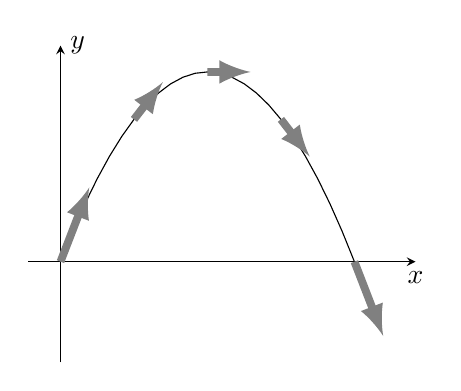
\begin{tikzpicture}[declare function={fx(\t)=\t;fy(\t)=\t-9.8/2*\t^2;gx(\t)=1;gy(\t)=1-9.8*\t;}]
\pgfmathsetmacro{\ta}{0.0*2/9.8}
\pgfmathsetmacro{\tb}{0.25*2/9.8}
\pgfmathsetmacro{\tc}{0.5*2/9.8}
\pgfmathsetmacro{\td}{0.75*2/9.8}
\pgfmathsetmacro{\te}{1.0*2/9.8}
\begin{axis}[clip=false,view/h=110,small,axis lines=middle,xtick={\empty},ytick={\empty},ztick={\empty},enlargelimits=true, xlabel={$x$}, ylabel={$y$},zlabel={$z$}, xlabel style={anchor=north},ylabel style={anchor=west},zlabel style={anchor=south},colormap={}{gray(0cm)=(0.6);gray(1cm)=(0.9);}]
\addplot[domain=0:2/9.8,variable =\t] ({fx(t)},{fy(t)});
\addplot[-latex,line width=1mm, gray]plot coordinates {({fx(\ta)},{fy(\ta)})({fx(\ta)+0.02*gx(\ta)},{fy(\ta)+0.02*gy(\ta)})};
\addplot[-latex,line width=1mm, gray]plot coordinates {({fx(\tb)},{fy(\tb)})({fx(\tb)+0.02*gx(\tb)},{fy(\tb)+0.02*gy(\tb)})};
\addplot[-latex,line width=1mm, gray]plot coordinates {({fx(\tc)},{fy(\tc)})({fx(\tc)+0.03*gx(\tc)},{fy(\tc)+0.02*gy(\tc)})};
\addplot[-latex,line width=1mm, gray]plot coordinates {({fx(\td)},{fy(\td)})({fx(\td)+0.02*gx(\td)},{fy(\td)+0.02*gy(\td)})};
\addplot[-latex,line width=1mm, gray]plot coordinates {({fx(\te)},{fy(\te)})({fx(\te)+0.02*gx(\te)},{fy(\te)+0.02*gy(\te)})};
\end{axis}
\end{tikzpicture}
\caption{گول انداز کے سمتی رفتار سمتیات \عددی{\kvec{v}(t)} سمتی میدان دیتے ہیں۔}
\label{شکل_سمتی_تکمل_سمتی_رفتار_میدان}
\end{figure}


\begin{figure}
\centering
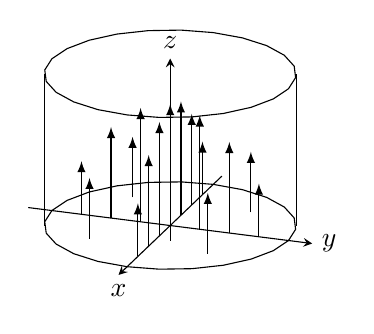
\begin{tikzpicture}[declare function={fx(\t)=cos(\t);fy(\t)=sin(\t);gz(\x,\y)=1-\x^2-\y^2;}]
\begin{axis}[clip=false,view/h=110,small,axis lines=middle,xtick={\empty},ytick={\empty},ztick={\empty},enlargelimits=true, xlabel={$x$}, ylabel={$y$},zlabel={$z$}, xlabel style={anchor=north},ylabel style={anchor=west},zlabel style={anchor=south},colormap={}{gray(0cm)=(0.6);gray(1cm)=(0.9);}]
\addplot3[domain=0:360,variable =\t] ({fx(t)},{fy(t)},{0});
\addplot3[domain=0:360,variable =\t] ({fx(t)},{fy(t)},{1.25});
\addplot3[]plot coordinates {({fx(110)},{fy(110)},{0})({fx(110)},{fy(110)},{1.25})};
\addplot3[]plot coordinates {({fx(110+180)},{fy(110+180)},{0})({fx(110+180)},{fy(110+180)},{1.25})};
\addplot3[-latex]plot coordinates {(0,0,0)(0,0,{gz(0,0)})};
\addplot3[-latex]plot coordinates {(-0.25,0,0)(-0.25,0,{gz(-0.25,0)})};
\addplot3[-latex]plot coordinates {(-0.5,0,0)(-0.5,0,{gz(-0.5,0)})};
\addplot3[-latex]plot coordinates {(-0.75,0,0)(-0.75,0,{gz(-0.75,0)})};
\addplot3[-latex]plot coordinates {(0.25,0,0)(00.25,0,{gz(0.25,0)})};
\addplot3[-latex]plot coordinates {(0.5,0,0)(00.5,0,{gz(0.5,0)})};
\addplot3[-latex]plot coordinates {(0.75,0,0)(00.75,0,{gz(0.75,0)})};
%
\addplot3[-latex]plot coordinates {(0,-0.25,0)(0,-0.25,{gz(0,-0.25)})};
\addplot3[-latex]plot coordinates {(0,-0.5,0)(0,-0.5,{gz(0,-0.5)})};
\addplot3[-latex]plot coordinates {(0,-0.75,0)(0,-0.75,{gz(0,-0.75)})};
\addplot3[-latex]plot coordinates {(0,0.25,0)(0,0.25,{gz(0,0.25)})};
\addplot3[-latex]plot coordinates {(0,0.5,0)(0,0.5,{gz(0,0.5)})};
\addplot3[-latex]plot coordinates {(0,0.75,0)(0,0.75,{gz(0,0.75)})};
%
\addplot3[-latex]plot coordinates {(-0.5,-0.5,0)(-0.5,-0.5,{gz(-0.5,-0.5)})};
\addplot3[-latex]plot coordinates {(0.5,-0.5,0)(0.5,-0.5,{gz(0.5,-0.5)})};
\addplot3[-latex]plot coordinates {(0.5,0.5,0)(0.5,0.5,{gz(0.5,0.5)})};
\addplot3[-latex]plot coordinates {(-0.5,0.5,0)(-0.5,0.5,{gz(-0.5,0.5)})};
\end{axis}
\end{tikzpicture}
\caption{
لمبی نالی میں سیال کی حرکت۔ مستوی \عددی{xy} میں  سمتیات \عددی{\kvec{v}=(a^2-\rho^2)\ak} کی دم اور قطع مکافی \عددی{z=a^2-\rho^2} پر  سر پائے جاتے ہیں۔
}
\label{شکل_سمتی_تکمل_نلکی_میں_بہاو_سیال}
\end{figure}


\begin{figure}
\centering
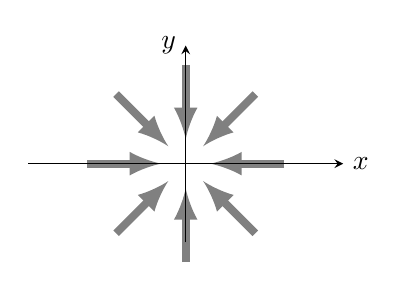
\begin{tikzpicture}[declare function={fx(\x,\y)=-0.75*\x;fy(\x,\y)=-0.75*\y;}]
\pgfmathsetmacro{\ka}{1.25}
\pgfmathsetmacro{\kr}{\ka/sqrt(2)}
\draw[-latex,gray,line width=1mm](\ka,0)--++({fx(\ka,0)},{fy(\ka,0)});
\draw[-latex,gray,line width=1mm](\kr,\kr)--++({fx(\kr,\kr)},{fy(\kr,\kr)});
\draw[-latex,gray,line width=1mm](-\ka,0)--++({fx(-\ka,0)},{fy(-\ka,0)});
\draw[-latex,gray,line width=1mm](0,\ka)--++({fx(0,\ka)},{fy(0,\ka)});
\draw[-latex,gray,line width=1mm](0,-\ka)--++({fx(0,-\ka)},{fy(0,-\ka)});
\draw[-latex,gray,line width=1mm](-\kr,-\kr)--++({fx(-\kr,-\kr)},{fy(-\kr,-\kr)});
\draw[-latex,gray,line width=1mm](\kr,-\kr)--++({fx(\kr,-\kr)},{fy(\kr,-\kr)});
\draw[-latex,gray,line width=1mm](-\kr,\kr)--++({fx(-\kr,\kr)},{fy(-\kr,\kr)});
\draw[-stealth](-2,0)--(2,0)node[right]{$x$};
\draw[-stealth](0,-1)--(0,1.5)node[left]{$y$};
\end{tikzpicture}
\caption{ثقلی میدان \عددی{\kvec{F}=-\tfrac{GM(x\ai+y\aj+z\ak)}{(x^2+y^2+z^2)^{3/2}}} میں سمتیات۔
}
\label{شکل_سمتی_تکمل_ثقلی_میدان}
\end{figure}


\begin{figure}
\centering
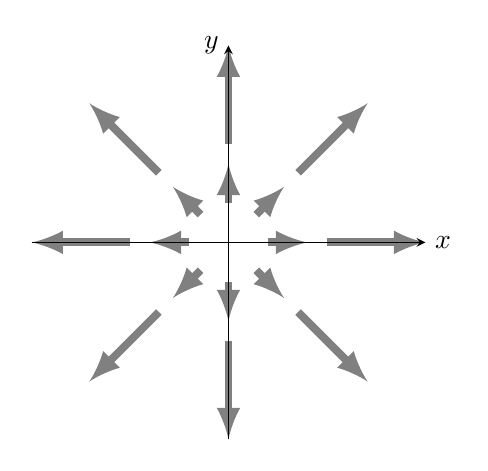
\begin{tikzpicture}[declare function={fx(\x,\y)=\x;fy(\x,\y)=\y;}]
\pgfmathsetmacro{\ka}{0.5}
\pgfmathsetmacro{\kr}{\ka/sqrt(2)}
\draw[-latex,gray,line width=1mm](\ka,0)--++({fx(\ka,0)},{fy(\ka,0)});
\draw[-latex,gray,line width=1mm](-\ka,0)--++({fx(-\ka,0)},{fy(-\ka,0)});
\draw[-latex,gray,line width=1mm](0,\ka)--++({fx(0,\ka)},{fy(0,\ka)});
\draw[-latex,gray,line width=1mm](0,-\ka)--++({fx(0,-\ka)},{fy(0,-\ka)});
\draw[-latex,gray,line width=1mm](\kr,\kr)--++({fx(\kr,\kr)},{fy(\kr,\kr)});
\draw[-latex,gray,line width=1mm](\kr,-\kr)--++({fx(\kr,-\kr)},{fy(\kr,-\kr)});
\draw[-latex,gray,line width=1mm](-\kr,\kr)--++({fx(-\kr,\kr)},{fy(-\kr,\kr)});
\draw[-latex,gray,line width=1mm](-\kr,-\kr)--++({fx(-\kr,-\kr)},{fy(-\kr,-\kr)});
\pgfmathsetmacro{\ka}{1.25}
\pgfmathsetmacro{\kr}{\ka/sqrt(2)}
\draw[-latex,gray,line width=1mm](\ka,0)--++({fx(\ka,0)},{fy(\ka,0)});
\draw[-latex,gray,line width=1mm](-\ka,0)--++({fx(-\ka,0)},{fy(-\ka,0)});
\draw[-latex,gray,line width=1mm](0,\ka)--++({fx(0,\ka)},{fy(0,\ka)});
\draw[-latex,gray,line width=1mm](0,-\ka)--++({fx(0,-\ka)},{fy(0,-\ka)});
\draw[-latex,gray,line width=1mm](\kr,\kr)--++({fx(\kr,\kr)},{fy(\kr,\kr)});
\draw[-latex,gray,line width=1mm](\kr,-\kr)--++({fx(\kr,-\kr)},{fy(\kr,-\kr)});
\draw[-latex,gray,line width=1mm](-\kr,\kr)--++({fx(-\kr,\kr)},{fy(-\kr,\kr)});
\draw[-latex,gray,line width=1mm](-\kr,-\kr)--++({fx(-\kr,-\kr)},{fy(-\kr,-\kr)});
\draw[-stealth](-2.5,0)--(2.5,0)node[right]{$x$};
\draw[-stealth](0,-2.5)--(0,2.5)node[left]{$y$};
\end{tikzpicture}
\caption{
مستوی میں مختلف نقاط پر  رداسی میدان \عددی{\kvec{F}=x\ai+y\aj} جہاں تیر دار لکیر کی دم اس نقطہ پر رکھی جاتی ہے جہاں کا سمتیہ درکار ہو۔
}
\label{شکل_سمتی_تکمل_رداسی_میدان}
\end{figure}



\begin{figure}
\centering
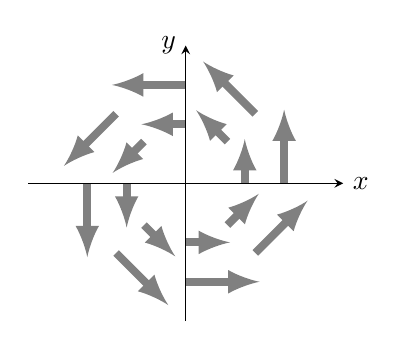
\begin{tikzpicture}[declare function={fx(\x,\y)=-0.75*\y;fy(\x,\y)=0.75*\x;}]
\pgfmathsetmacro{\ka}{0.75}
\pgfmathsetmacro{\kr}{\ka/sqrt(2)}
\draw[-latex,gray,line width=1mm](\ka,0)--++({fx(\ka,0)},{fy(\ka,0)});
\draw[-latex,gray,line width=1mm](-\ka,0)--++({fx(-\ka,0)},{fy(-\ka,0)});
\draw[-latex,gray,line width=1mm](0,\ka)--++({fx(0,\ka)},{fy(0,\ka)});
\draw[-latex,gray,line width=1mm](0,-\ka)--++({fx(0,-\ka)},{fy(0,-\ka)});
\draw[-latex,gray,line width=1mm](\kr,\kr)--++({fx(\kr,\kr)},{fy(\kr,\kr)});
\draw[-latex,gray,line width=1mm](\kr,-\kr)--++({fx(\kr,-\kr)},{fy(\kr,-\kr)});
\draw[-latex,gray,line width=1mm](-\kr,\kr)--++({fx(-\kr,\kr)},{fy(-\kr,\kr)});
\draw[-latex,gray,line width=1mm](-\kr,-\kr)--++({fx(-\kr,-\kr)},{fy(-\kr,-\kr)});
\pgfmathsetmacro{\ka}{1.25}
\pgfmathsetmacro{\kr}{\ka/sqrt(2)}
\draw[-latex,gray,line width=1mm](\ka,0)--++({fx(\ka,0)},{fy(\ka,0)});
\draw[-latex,gray,line width=1mm](-\ka,0)--++({fx(-\ka,0)},{fy(-\ka,0)});
\draw[-latex,gray,line width=1mm](0,\ka)--++({fx(0,\ka)},{fy(0,\ka)});
\draw[-latex,gray,line width=1mm](0,-\ka)--++({fx(0,-\ka)},{fy(0,-\ka)});
\draw[-latex,gray,line width=1mm](\kr,\kr)--++({fx(\kr,\kr)},{fy(\kr,\kr)});
\draw[-latex,gray,line width=1mm](\kr,-\kr)--++({fx(\kr,-\kr)},{fy(\kr,-\kr)});
\draw[-latex,gray,line width=1mm](-\kr,\kr)--++({fx(-\kr,\kr)},{fy(-\kr,\kr)});
\draw[-latex,gray,line width=1mm](-\kr,-\kr)--++({fx(-\kr,-\kr)},{fy(-\kr,-\kr)});
\draw[-stealth](-2,0)--(2,0)node[right]{$x$};
\draw[-stealth](0,-1.75)--(0,1.75)node[left]{$y$};
\end{tikzpicture}
\caption{اکائی سمتیات \عددی{\kvec{F}=\tfrac{-y\ai+x\aj}{\sqrt{x^2+y^2}}} کا چکری میدان۔}
\label{شکل_سمتی_تکمل_چکری_میدان}
\end{figure}

\begin{figure}
\centering
\begin{tikzpicture}
%\draw[step=1,thick,black] (0,0) grid (6,2);
%\draw[xstep=0.1,ystep=0.1,thin] (0,0) grid (6,2);
\draw(0,0)node[circ]{}node[above,xshift=-1ex]{$A$}node[right]{$t=a$}to [out=45, in=180](3,2) to [out=0,in=90](4,1)to [out=-90,in=0](3,0) to [out=180,in=180](3,1.5)to [out=0,in=135](3.95,1)  (4.05,0.9) to [out=-45,in=180](5,0)to[out=0,in=-135](6,1)node[circ]{}node[above]{$B$}node[right]{$t=b$};
\draw[-latex](3.72,1.7)node[circ]{}--++(-50:1)node[right]{$\kvec{T}$};
\draw[-latex](3.72,1.7)--++(10:0.75)node[right]{$\kvec{F}$};
\end{tikzpicture}
\caption{
ہموار راہ \عددی{\kvec{r}(t)=g(t)\ai+h(t)\aj+k(t)\ak} پر \عددی{A} سے \عددی{B} تک استمراری قوت \عددی{\kvec{F}} کا کام \عددی{t=a} تا \عددی{t=b} راہ کی ہمراہ \عددی{\kvec{F}\cdot\kvec{T}} کا تکمل ہو گا۔
}
\label{شکل_سمتی_تکمل_کام_کی_تعریف_مستقل_قوت}
\end{figure}


\begin{figure}
\centering
\begin{tikzpicture}[font=\small,declare function={fx(\x)=-sin(\x);}]
\coordinate (O) at (0,0);
\draw[smooth, domain=0:200]plot ({\x/30},{fx(\x)});
\foreach \t in {0,6,9,20}{\path[| mark=0.5] ({(\t-0.1)/3},{fx((\t-0.1)*10)}) -- ({(\t+0.1)/3},{fx((\t+0.1)*10)});}
\draw[]plot ({70/30},{fx(70)})node[circ]{}node[below,xshift=1ex]{$t=c_k$};
\draw[]plot ({0/30},{fx(0)})node[above]{$t=t_a$};
\draw[]plot ({200/30},{fx(200)})node[above]{$t=t_b$};
\draw[]plot ({60/30},{fx(60)})node[pin=-135:{$N_k(g(t_k),h(t_k),k(t_k))$}]{};
\draw[]plot ({90/30},{fx(90)})node[pin=-45:{$N_{k+1}(g(t_{k+1}),h(t_{k+1}),k(t_{k+1}))$}]{};
\draw[decorate,decoration={brace,amplitude=5pt, raise=5pt}] ({60/30},{fx(60)})--({90/30},{fx(90)})node[pos=0.5,above,shift={(60:0.3)}]{$\Delta s_k$};
\draw[] (1,1)--(5,1);
\path[| mark=0] ({1},{1})node[below]{$a$} -- ({1+0.1},{1});
\path[| mark=0] ({5},{1})node[below]{$b$} -- ({5+0.1},{1});
\path[| mark=0] ({60/30},{1})node[below]{$t_k$} -- ({62/30},{1});
\path[| mark=0] ({90/30},{1})node[below]{$t_{k+1}$} -- ({92/30},{1});
\draw ({70/30},{1})node[circ]{}node[above]{$c_k$};
\draw[]plot ({150/30},{fx(150)})node[above]{$\kvec{r}$};
\end{tikzpicture}
\caption{
مقدار معلوم وقفہ \عددی{a\le t\le b} کی ہر خانہ بندی منحنی \عددی{\kvec{r}=g(t)\ai+h(t)\aj+k(t)\ak} کی خانہ بندی پیدا کرتی ہے۔  
}
\label{شکل_سمتی_تکمل_خانہ_بندی_اور_تفاعل}
\end{figure}



\begin{figure}
\centering
\begin{tikzpicture}[font=\small,declare function={fx(\x)=-3*sin(\x);}]
\coordinate (O) at (0,0);
\draw[smooth, domain=55:95]plot ({\x/10},{fx(\x)});
\foreach \t/\pos/\l in {6/below/{N_k},9/above/{N_{k+1}}}{\path[| mark=0.5] ({(\t-0.1)},{fx((\t-0.1)*10)}) -- ({(\t+0.1)},{fx((\t+0.1)*10)})node[pos=0.5,\pos]{$\l$};}
\draw[]({70/10},{fx(70)})node[circ]{}node[pin=100:{$t=c_k$}]{};
\draw[-latex] ({70/10},{fx(70)})--++(30:1.25)coordinate(kT)node[pos=0.75,above left]{$\kvec{F}_k$};
\draw[-latex] ({70/10},{fx(70)})coordinate(kL)--++(-10:1.75)coordinate(kR)node[below]{$\kvec{T}_k$};
\draw[dashed](kT)--($(kL)!(kT)!(kR)$)coordinate(kM);
\draw[decorate,decoration={brace,amplitude=5pt, raise=5pt}] (kM)--(kL)node[pos=0.5,below,shift={(-90:0.3)}]{$\kvec{F}_k\cdot\kvec{T}_k$};
\end{tikzpicture}
\caption{
گزشتہ شکل کے  قطع \عددی{N_kN_{k+1}} کو بڑا کر کے \عددی{t=c_k} کے مطابقتی نقطہ پر اکائی مماسی سمتیہ \عددی{\kvec{T}} اور قوت سمتیہ \عددی{\kvec{F}} دکھائے گئے ہیں۔   
}
\label{شکل_سمتی_تکمل_خانہ_بندی_تفصیل}
\end{figure}


\begin{figure}
\centering
\begin{tikzpicture}[declare function={fx(\t)=\t;fy(\t)=\t^2;fz(\t)=\t^3;}]
\begin{axis}[clip=false,view/h=110,small,axis lines=middle,xtick={\empty},ytick={\empty},ztick={\empty},enlargelimits=true, xlabel={$x$}, ylabel={$y$},zlabel={$z$}, xlabel style={anchor=east},ylabel style={anchor=west},zlabel style={anchor=south},colormap={}{gray(0cm)=(0.6);gray(1cm)=(0.9);}]
\addplot3[domain=0:1,variable =\t,samples y=0]({fx(t)},{fy(t)},{fz(t)})node[circ]{}node[right]{$(1,1,1)$}node[pos=0.8,pin={[fill=white]110:{$\kvec{r}=t\ai+t^2\aj+t^3\ak$}}]{};
\addplot3[dashed]plot coordinates {({fx(1)},{fy(1)},{fz(1)})({fx(1)},{fy(1)},{0})({0},{fy(1)},{0})};
\addplot3[dashed]plot coordinates {({fx(1)},{fy(1)},{0})({fx(1)},{0},{0})}node[pos=0,right,yshift=-1ex]{$(1,1,0)$};
\end{axis}
\end{tikzpicture}
\caption{}
\label{شکل_مثال_سمتی_تکمل_منحنی_قوسی}
\end{figure}

\begin{figure}
\centering
\begin{subfigure}{0.45\textwidth}
\centering
\begin{tikzpicture}[declare function={fx(\t)=3+2*cos(\t);fy(\t)=1.5+sin(\t);fz(\t)=0;}]
\begin{axis}[clip=false,view/h=110,small,axis lines=middle,xtick={\empty},ytick={\empty},ztick={\empty},enlargelimits=true, xlabel={$x$}, ylabel={$y$},zlabel={$z$}, xlabel style={anchor=east},ylabel style={anchor=west},zlabel style={anchor=south},colormap={}{gray(0cm)=(0.6);gray(1cm)=(0.9);},zmin=0,zmax=0.75]
\addplot3[,-<-=0.25,-<-=0.75,domain=0:360,variable =\t,samples y=0]({fx(t)},{fy(t)},{fz(t)})node[pos=0.25,right]{$C$};
\addplot3[-latex]plot coordinates {({fx(0)},{fy(0)},{fz(0)})({fx(0)},{fy(0)},{0.25})}node[pos=0.75,right]{$\ak$};
\addplot3[-latex]plot coordinates {({fx(0)},{fy(0)},{fz(0)})(5,0.75,0)}node[below]{$\kvec{T}$};
\addplot3[-latex]plot coordinates {({fx(0)},{fy(0)},{fz(0)})(7,1.5,0)}node[below]{$\ak\times \kvec{T}$};
\end{axis}
\end{tikzpicture}
\caption{گھڑی وار حرکت کے لئے \عددی{\ak\times\kvec{T}} باہر رخ ہو گا۔}
\end{subfigure}\hfill
\begin{subfigure}{0.45\textwidth}
\centering
\begin{tikzpicture}[declare function={fx(\t)=3+2*cos(\t);fy(\t)=1.5+sin(\t);fz(\t)=0;}]
\begin{axis}[clip=false,view/h=110,small,axis lines=middle,xtick={\empty},ytick={\empty},ztick={\empty},enlargelimits=true, xlabel={$x$}, ylabel={$y$},zlabel={$z$}, xlabel style={anchor=east},ylabel style={anchor=west},zlabel style={anchor=south},colormap={}{gray(0cm)=(0.6);gray(1cm)=(0.9);},zmin=0,zmax=0.75]
\addplot3[,->-=0.25,->-=0.75,domain=0:360,variable =\t,samples y=0]({fx(t)},{fy(t)},{fz(t)})node[pos=0.25,right]{$C$};
\addplot3[-latex]plot coordinates {({fx(0)},{fy(0)},{fz(0)})({fx(0)},{fy(0)},{0.25})}node[pos=0.75,right]{$\ak$};
\addplot3[-latex]plot coordinates {({fx(0)},{fy(0)},{fz(0)})(5,2.25,0)}node[below]{$\kvec{T}$};
\addplot3[-latex]plot coordinates {({fx(0)},{fy(0)},{fz(0)})(7,1.5,0)}node[below]{$\kvec{T}\times \ak$};
\end{axis}
\end{tikzpicture}
\caption{خلاف گھڑی حرکت کے لئے \عددی{\kvec{T}\times\ak} باہر رخ ہو گا۔}
\end{subfigure}
\caption{
ہموار منحنی \عددی{C}، جو بڑھتے \عددی{t} کی صورت میں مستوی \عددی{xy} میں  خلاف گھڑی حرکت کرتی ہو،  کا باہر رخ اکائی
 سمتیہ \عددی{\kvec{n}=\kvec{T}\times\ak} ہو گا۔
}
\label{شکل_سمتی_تکمل_گھڑی_وار}
\end{figure}

\begin{figure}
\centering
\begin{tikzpicture}[declare function={fx(\t)=\t;fy(\t)=\t^2;fz(\t)=\t^3;}]
\begin{axis}[clip=false,view/h=110,small,axis lines=middle,xtick={\empty},ytick={\empty},ztick={\empty},enlargelimits=true, xlabel={$x$}, ylabel={$y$},zlabel={$z$}, xlabel style={anchor=east},ylabel style={anchor=west},zlabel style={anchor=south},colormap={}{gray(0cm)=(0.6);gray(1cm)=(0.9);}]
\addplot3[domain=0:1,variable =\t,samples y=0]({fx(t)},{fy(t)},{fz(t)})node[circ]{}node[right]{$(1,1,1)$}node[pos=0.25,below]{$C_2$}node[pos=0,above left]{$(0,0,0)$};
\addplot3[]plot coordinates {({fx(1)},{fy(1)},{fz(1)})({fx(1)},{fy(1)},{0})}node[pos=0.6,right]{$C_4$};
\addplot3[dashed]plot coordinates {({fx(1)},{fy(1)},{0})({0},{fy(1)},{0})};
\addplot3[dashed]plot coordinates {({fx(1)},{fy(1)},{0})({fx(1)},{0},{0})}node[pos=0,right,yshift=-1ex]{$(1,1,0)$};
\addplot3[]plot coordinates {(0,0,0)({fx(1)},{fy(1)},{0})}node[pos=0.5,below]{$C_3$};
\addplot3[]plot coordinates {(0,0,0)({fx(1)},{fy(1)},{fz(1)})}node[pos=0.5,above]{$C_1$};
\end{axis}
\end{tikzpicture}
\caption{}
\label{شکل_سمتی_تکمل_ایک_نقطہ_سے_دوسری_تک_راہ}
\end{figure}


\begin{figure}
\centering
\begin{tikzpicture}[declare function={fx(\t)=cos(deg(\t));fy(\t)=sin(deg(\t));fz(\t)=\t;}]
\begin{axis}[clip=false,view/h=110,small,axis lines=middle,xtick={\empty},ytick={\empty},ztick={\empty},enlargelimits=true, xlabel={$x$}, ylabel={$y$},zlabel={$z$}, xlabel style={anchor=north},ylabel style={anchor=north},zlabel style={anchor=south},colormap={}{gray(0cm)=(0.6);gray(1cm)=(0.9);},xmax=1.25]
\addplot3[->-=0.85,domain=0:pi/2,variable =\t,samples y=0]({fx(t)},{fy(t)},{fz(t)})node[circ]{}node[right]{$(0,1,\tfrac{\pi}{2})$}node[pos=0.75,below]{$C_1$}node[pos=0,circ]{}node[pos=0,left]{$(1,0,0)$};
\addplot3[->-=0.5]plot coordinates {({fx(pi/2)},{fy(pi/2)},{fz(pi/2)})({fx(pi/2)},{fy(pi/2)},{0})}node[pos=0.5,right]{$C_2$}node[pos=1,above right]{$(0,1,0)$};
\addplot3[->-=0.5]plot coordinates {({fx(pi/2)},{fy(pi/2)},{0})({1},{0},{0})}node[pos=0.75,below]{$C_3$}node[pos=1,left]{$(1,0,0)$};
\end{axis}
\end{tikzpicture}
\caption{}
\end{figure}


\begin{figure}
\centering
\begin{tikzpicture}[declare function={fx(\t)=\t;fy(\t)=\t^2;gx(\x)=\x;gz(\x)=\x;}]
\pgfmathsetmacro{\k}{0.4}
\pgfmathsetmacro{\ks}{1}
\pgfmathsetmacro{\ke}{1}
\begin{axis}[clip=false,view={80}{30},small,axis lines=middle,xtick={\empty},ytick={\empty},ztick={\empty},enlargelimits=true, xlabel={$x$}, ylabel={$y$},zlabel={$z$}, xlabel style={anchor=north},ylabel style={anchor=north},zlabel style={anchor=east},colormap={}{gray(0cm)=(0.6);gray(1cm)=(0.9);},xmin=0,ymin=-1.25,zmin=0]
\addplot3[domain=-\ks:\ke,variable =\t,samples y=0]({fx(t)},{fy(t)},{0});
\addplot3[domain=-\ks:\ke,variable =\t,samples y=0]({fx(t)},{fy(t)},{1})node[pos=0,right]{$y=x^2$};
\addplot3[]plot coordinates {({fx(-\ks)},{fy(-\ks)},{0})({fx(-\ks)},{fy(-\ks)},{1})};
\addplot3[]plot coordinates {({fx(\ke)},{fy(\ke)},{0})({fx(\ke)},{fy(\ke)},{1})};
\addplot3[]plot coordinates {(-1,-1,-1)(1,-1,1) (1,2,1) (-1,2,-1)(-1,-1,-1)};
\addplot3[->-=0.5,domain=0:1,thick,samples y=0]({x},{x^2},{x})node[circ]{}node[above,xshift=2ex]{$(1,1,1)$};
\addplot3[]plot coordinates {(1,2,1)}node[right]{$z=x$};
\end{axis}
\end{tikzpicture}
\caption{}
\end{figure}


\begin{figure}
\centering
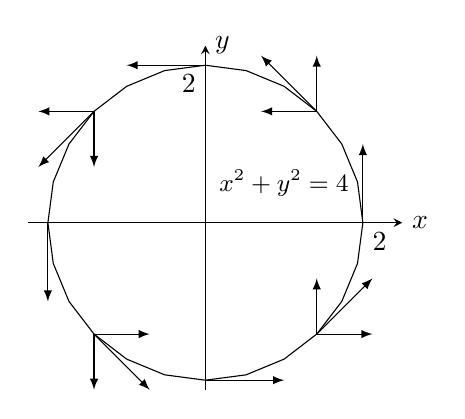
\begin{tikzpicture}[declare function={fx(\x,\y)=-\y/sqrt((\x)^2+(\y)^2);fy(\x,\y)=\x/sqrt((\x)^2+(\y)^2);gx(\t)=2*cos(\t);gy(\t)=2*sin(\t);}]
\pgfmathsetmacro{\k}{2}
\pgfmathsetmacro{\kk}{\k*cos(45)}
\draw[-stealth](-2.25,0)--(2.5,0)node[right]{$x$};
\draw[-stealth](0,-2.125)--(0,2.25)node[right]{$y$};
\draw[domain=0:360] plot ({gx(\x)},{gy(\x)});
\draw[-latex](\k,0)node[below right]{$2$}--++({fx(\k,0)},{fy(\k,0)});
\draw[-latex](-\k,0)--++({fx(-\k,0)},{fy(-\k,0)});
\draw[-latex](0,\k)node[below left]{$2$}--++({fx(0,\k)},{fy(0,\k)});
\draw[-latex](0,-\k)--++({fx(0,-\k)},{fy(0,-\k)});
%
\draw[-latex](\kk,\kk)--++({fx(\kk,\kk)},{fy(\kk,\kk)});
\draw[-latex](-\kk,\kk)--++({fx(-\kk,\kk)},{fy(-\kk,\kk)});
\draw[-latex](\kk,-\kk)--++({fx(\kk,-\kk)},{fy(\kk,-\kk)});
\draw[-latex](-\kk,-\kk)--++({fx(-\kk,-\kk)},{fy(-\kk,-\kk)});
%
\draw[-latex](\kk,\kk)--++({fx(\kk,\kk)},{0});
\draw[-latex](\kk,\kk)--++({0},{fy(\kk,\kk)});
\draw[-latex](-\kk,\kk)--++({fx(-\kk,\kk)},{0});
\draw[-latex](-\kk,\kk)--++({0},{fy(-\kk,\kk)});
\draw[-latex](\kk,-\kk)--++({fx(\kk,-\kk)},{0});
\draw[-latex](\kk,-\kk)--++({0},{fy(\kk,-\kk)});
\draw[-latex](-\kk,-\kk)--++({fx(-\kk,-\kk)},{0});
\draw[-latex](-\kk,-\kk)--++({0},{fy(-\kk,-\kk)});
\draw(1,0.5)node[font=\small]{$x^2+y^2=4$};
\end{tikzpicture}
\caption{}
\end{figure}

